\documentclass[12pt,a4paper]{article}
\usepackage[polish]{babel}
\usepackage[T1]{fontenc}
\usepackage[utf8x]{inputenc}
\usepackage{hyperref}
\usepackage{url}
\usepackage{graphicx}

\addtolength{\hoffset}{-1.5cm}
\addtolength{\marginparwidth}{-1.5cm}
\addtolength{\textwidth}{3cm}
\addtolength{\voffset}{-1cm}
\addtolength{\textheight}{2.5cm}
\setlength{\topmargin}{0cm}
\setlength{\headheight}{0cm}

\begin{document}

\title{Dokumentacja projektu ZPI}
\author{Dąbrowski Daniel\\ Gródek Damian\\ Jargut Piotr\\ Kocjan Katarzyna\\ Uryga Kamil}
\date{\today}

\maketitle

\begin{abstract}
Zarys dokumentacji projektowej stanowiący podstawę do realizacji projektu \\ zespołowego. 
\end{abstract}



\newpage

\tableofcontents
\listoftables
\listoffigures



\newpage

\section{Tytuł: System wspomagający szybkie parkowanie}

\section{Nazwa robocza: Parkingowy}

\section{Cel}
\begin{quotation}
Zoptymalizować ruch na parkingach i zniwelować długi czas szukania miejsca parkingowego, co pozwoli na zmniejszenie emisji spalin do atmosfery.
\end{quotation}
\begin{quotation}
Przewidywany termin ukończenia projektu 10 Maja.
\end{quotation}

\section{Zakres}

\subsection{Analiza wymagań}

{\large \bf System :}
\begin{itemize}
\item Określenie optymalnego położenia emiterów beacon na podstawie planu parkingu \\i zasięgu emiterów;
\item Instalacja serwera;
\item Stworzenie bazy danych i szkieletu aplikacji;
\item Implementacja systemu zarządzania wolnymi  miejscami;
\item Instalacja Acess pointów wifi mesh z funkcją emitera beacon;
\item Implementacja funkcji lokalizacji telefonu na terenie parkingu;
\item Implementacja systemu komunikacji pomiędzy czujnikami zajętości miejsca a serwerem za pośrednictwem protokołu MQTT;
\item Implementacja funkcji sugerowania wolnych miejsc parkingowych;
\item Rozmieszczenie czujników zajętości miejsca;
\item Implementacja systemu komunikacji pomiędzy szlabanami a serwerem;
\item Testy;
\item Gotowy system.
\end{itemize}
{\large \bf Użytkownik :}

{\bf Aplikacja:}
\begin{itemize}
\item System lokalizacji;
\item System rejestracji;
\item System logowania do aplikacji;
\item Gotowy system.
\end{itemize}



\newpage

{\bf System wspomagający parkowanie:}
\begin{itemize}
\item System zarządzający wolnymi miejscami;
\item System sygnałów świetlnych.
\end{itemize}

{\bf System lokalizacji pojazdu na parkingu:}
\begin{itemize}
\item System nawigacji do samochodu;
\item Zapamiętanie lokalizacji samochodu.
\end{itemize}
{\large \bf Administrator :}
\begin{itemize}
\item Gotowe rozmieszczenie urządzeń/sprzętu;
\item Gotowe rozmieszczenie czujników;
\item Gotowe połączenia bezprzewodowe z urządzeniami i serwerem na celu serwisu i identyfikacji wymiany baterii bądź naprawy czujników.
\end{itemize}

\subsection{Wymagania funkcjonalne i niefunkcjonalne}
{\large \bf Wymagania funkcjonalne :}
\\Użytkownik ma możliwość :
\begin{itemize}
\item Sprawdzenia ilości wolnych miejsc;
\item Sprawdzenia ilości zajętych miejsc;
\item Poinformowaniu o ewentualnym braku miejsc na danym piętrze;
\item Poinformowaniu o zwolnieniu najbliższego wolnego miejsca;
\item Aplikacja sugeruje najbliższe wolne miejsce parkingowe;
\item System kieruje kierowcę systemem świateł.
\end{itemize}
{\large \bf Wymagania niefunkcjonalne:}
\begin{itemize}
\item Aplikacja powinna być darmowa;
\item Aplikacja powinna mieć intuicyjny i przejrzysty interfejs;
\item Aplikacja powinna być kompatybilna z większością urządzeń aby mogło używać jej jak najwięcej użytkowników.
\end{itemize}



\newpage

\subsection{Diagram przypadków użycia i diagram przepływu (opcjonalny)}
\begin{figure}[htb!p]
\begin{center}
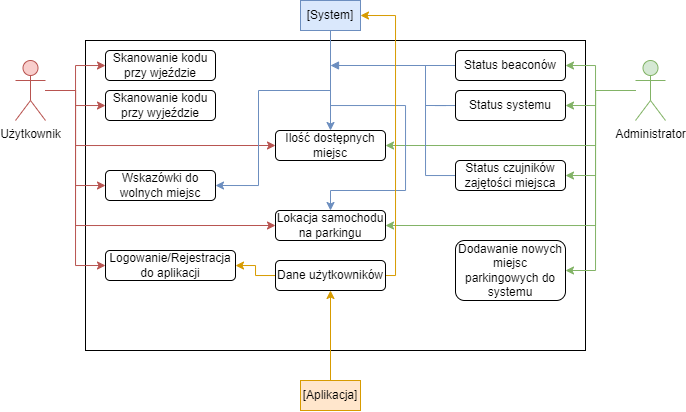
\includegraphics[width=0.9\textwidth]{Untitled_Diagram.drawio_1.png}
\caption{Diagram przypadków użycia}
\end{center}
\end{figure}

\subsection{Dobór technologii}
\begin{itemize}
\item Emitery beacon pracujące na protokole BT low energy(Access point’y zintegrowane \\z emiterami Beacon);
\item Magnetyczne czujniki zajętości miejsca (wifi, MQTT);
\item Windows Server;
\item Broker MQTT (RabitMQTT, Mosquito);
\item Android Studio(język JAVA);
\item Node-RED;
\item MSSQL;
\item ASP NET 4.8  (C\#).
\end{itemize}



\newpage

\section{Scenariusze}
{\large \bf Scenariusz:} Sugerowanie miejsca parkingowego
\\{\bf Nr:} 01
\\{\bf Aktor:} Użytkownik aplikacji
\\{\bf Stan wejścia:}

Warunek: Posiadanie aplikacji, znalezienie się przy wjeździe do parkingu.

Dane:
\\{\bf Przebieg scenariusza:}
\begin{enumerate}
\item Użytkownik dojeżdża na parking i skanuje aplikacje przy szlabanie na wjeździe;
\item Użytkownik otrzymuje sugestie kierujące go do miejsca parkingowego i parkuje;
\item System zmienia status miejsca parkingowego na zajęty.
\end{enumerate}
{\bf Wynik:} Użytkownik bez problemu parkuje swój pojazd.
\newline\newline
{\large \bf Scenariusz:} Zwolnienie miejsca parkingowego
\\{\bf Nr:} 02
\\{\bf Aktor:} Użytkownik aplikacji
\\{\bf Stan wejścia:}

Warunek: Użytkownik ma już zaparkowane auto na parkingu.

Dane:
\\{\bf Przebieg scenariusza:}
\begin{enumerate}
\item Użytkownik opuszcza miejsce parkingowe;
\item System wykrywa opuszczenie miejsca parkingowego przez auto i zmienia status miejsca na wolny;
\item Użytkownik skanuje aplikacje przy szlabanie na wyjeździe i wyjeżdza z parkingu.
\end{enumerate}
{\bf Wynik:} Użytkownik pouszcza parking.
\newline\newline\newline\newline\newline\newline\newline\newline\newline\newline\newline\newline\newline\newline\newline\newline
{\large \bf Scenariusz:} Lokalizacja zaparkowanego samochodu
\\{\bf Nr:} 03
\\{\bf Aktor:} Użytkownik aplikacji
\\{\bf Stan wejścia:}

Warunek: Użytkownik ma już zaparkowane auto na parkingu oraz ma zainstalowaną \\aplikację i zapisał w aplikacji miejsce w którym zaparkował.

Dane:
\\{\bf Przebieg scenariusza:}
\begin{enumerate}
\item Użytkownik wraca np z zakupów i zapomniał gdzie zaparkował;
\item Aplikacja pokazuje miejsce gdzie auto zostało zaparkowane;
\item Użytkownik znajduje swój pojazd i wyjeżdza z parkingu.
\end{enumerate}
{\bf Scenariusz alternatywny:}
\begin{enumerate}
\item Użytkownik nie zapisał pkt parkowania przez co aplikacja nie pokazuje lokalizacja;
\item Użytkownik jest zmuszony szukać swojego samochodu  bo nie zapisał lokalizacji gdzie zaparkował.
\end{enumerate}
{\bf Wynik:} Użytkownik znajduje swój pojazd i opuszcza parking.
\newline\newline\newline\newline\newline\newline\newline\newline\newline\newline\newline\newline\newline\newline\newline\newline\newline\newline\newline\newline\newline\newline\newline\newline\newline\newline
{\large \bf Scenariusz:} Rozładowanie telefonu
\\{\bf Nr:} 04
\\{\bf Aktor:} Użytkownik aplikacji
\\{\bf Stan wejścia:}

Warunek: Użytkownik ma już zaparkowane auto na parkingu.

Dane:
\\{\bf Przebieg scenariusza:}
\begin{enumerate}
\item Jeśli w czasie np zakupów użytkownikowi rozładuje się telefon nie będzie on w stanie wyjechać;
\item Jeśli nie jest sam może on zalogowac sie z innego telefonu(osoby towarzyszącej);
\item Użytkownik loguje się z innego telefonu pobiera aplikacje;
\item Po wpisaniu danych do aplikacji loguje się i może wyjechać.
\end{enumerate}
{\bf Scenariusz alternatywny 1:}
\begin{enumerate}
\item Jeżeli osoba jest sama i jeśli posiada ładowarke samochodową ładuje telefon aby móc uruchomić aplikację;
\item Użytkownik wyjeżdza z parkingu.
\end{enumerate}
{\bf Scenariusz alternatywny 2:}
\begin{enumerate}
\item Użytkownik nie posiada ładowarki samochodowej;
\item Użytkownik idzie do budki ochroniarskiej i przekazuje swoje dane do identyfikacji;
\item Użytkownik dostaje bilecik dzięki któremu wyjedzie a ochroniarz po jego wyjeździe wypisuje go z serwera żeby puścił parking;
\item Użytkownik wyjeżdza z parkingu.
\end{enumerate}
{\bf Wynik:} Użytkownik ponownie uzyskuje dostęp do aplikacji i opuszcza parking.
\newline\newline\newline\newline\newline\newline\newline\newline\newline\newline\newline\newline\newline\newline\newline
{\large \bf Scenariusz:} Wymiana baterii w czujnikach
\\{\bf Nr:} 05
\\{\bf Aktor:} Administrator
\\{\bf Stan wejścia:}

Warunek: Rozładowanie baterii w czujnikach.

Dane:
\\{\bf Przebieg scenariusza:}
\begin{enumerate}
\item Po ok 2 latach czujniki wysłały sygnał o zmianę baterii z powodu jej rozładowania;
\item Administrator wymienia w wymaganych czujnikach baterie.
\end{enumerate}
{\bf Wynik:} Czujniki działają dalej sprawnie dzięki wymienionym bateriom.
\newline\newline
{\large \bf Scenariusz:} Dodanie nowych miejsc parkingowych do systemu
\\{\bf Nr:} 06
\\{\bf Aktor:} Administrator
\\{\bf Stan wejścia:}

Warunek: Rozbudowa o nowe miejsca parkingowe.

Dane:
\\{\bf Przebieg scenariusza:}
\begin{enumerate}
\item Administrator konfiguruje nowe czujniki i odczytuje UID;
\item Administrator dodaje czujniki do node red’a i tworzy zapytania SQL;
\item Administrator tworzy nowe rekordy w bazie danych;
\item Rozbudowanie aplikacji.
\end{enumerate}
{\bf Wynik:} Aplikacja zostaje zaktualizowana, a baza danych zwiększona o nowe rekordy.



\newpage

\section{Estymacja czasowa}
\begin{figure}[htb!p]
\begin{center}
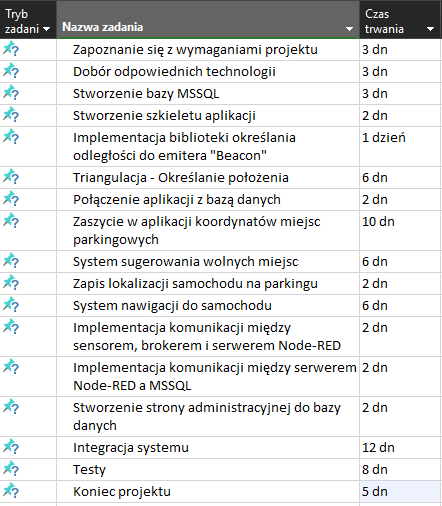
\includegraphics[width=0.7\textwidth]{unknown.png}
\caption{Estymacja czasowa}
\end{center}
\end{figure}



















%(poszczególnych zadań jak i określenie wymagań MVP oraz terminu końcowego oddania)
%\section{Implementacja}
%\section{Testy i ich wyniki}
%\section{Podsumowanie i bilans}
%(MVP vs rzeczywistość)
\end{document}